\documentclass[a4paper]{article}
\usepackage[utf8]{inputenc}
\usepackage[T1]{fontenc}
\usepackage{lmodern}
\usepackage[magyar]{babel}
\usepackage{cite}
\usepackage{graphicx}
\usepackage[font=footnotesize,labelfont=bf]{caption}
\graphicspath{ {./figures/} }
\usepackage{hyperref}
\hypersetup{
	colorlinks=true,
	linkcolor=black,
	filecolor=magenta,      
	urlcolor=cyan,
	citecolor=black,
}
\title{Májszegmentáció \linebreak konvolúciós neurális hálók segítségével}
\author{Kiss Benedek Gábor\and Németh Zoltán\and Szűcs Tamás }
\begin{document}
	\maketitle
	\tableofcontents
	\section*{Bevezető}
	Az orvosi tudományterületen egyre nagyobb mértékben kezdik el a különböző Big Data megoldások alkalmazását kutatni.\cite{2019arXiv190903029S}. Ezen technikák gyakorlatba való átültetése nagyban segítené a modern egészségügyet jó néhány problémájának megoldásában, többek között minimalizálni tudná az emberi hibákat és tehermentesíteni a túlterhelt egészségügyi dolgozókat. A félév során egy májszegmentációs neurális háló felépítését, és betanítását tűztük ki célul, abeli reménnyel, hogy később az eredmények felhasználásával májtumor szegmentációt tudjunk végezni. A téma kidolgozása során implementálásra került egy saját Python modul, ami egy paraméterezhető V-Net architektúrát valósít meg, ezen kívül egy három dimenziós augmentációt megvalósító Python modul.
	\pagebreak
	\section{Módszertan}
	Ez a szekció részletezi a félév során végrehajtott munkát. A  a pontos megvalósítások elérhetőek a \url{https://github.com/Biomfire/temalab_main} címen.\\
	\subsection{Adatok}
	\begin{figure}
		\centering
		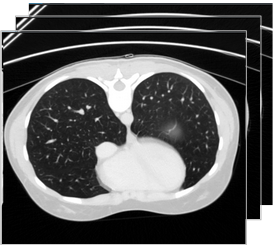
\includegraphics[width=0.45\linewidth]{figures/LiverInputSample}
		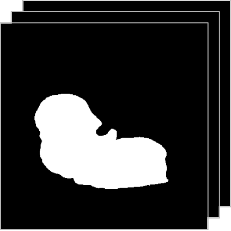
\includegraphics[width=0.45\linewidth]{figures/MaskInputSample}
		\caption{Tanításhoz használt adatok}
		\label{fig:liverinputsample}
	\end{figure}
	Az adathalmaz a Semmelweis Egyetem által biztosított 62 db Nifti formátumú CT felvétel és az ezekhez tartozó maszkok (\ref{fig:liverinputsample}. ábra). Ezek a fájlok átlagosan 30, de minimum 21 db, 512$\times$512 voxeles szeletet tartalmaztak. A kapott adathalmaz a Z-tengely menti eltérések kivételével normalizálva volt, a felvételek nagyjából a tüdő alsó részétől, a medence felső részéig tartottak. A maszkon a fehérrel jelölt területen a máj található, a feketével jelölt terület pedig a többi szervet jelölte.\\
	%TODO lehivatkozni
	\subsection{Az adatok augmentálása}
	A rendelkezésre álló adatok mennyisége a hagyományos Machine Learning-ben alkalmazott adatbázisok méretéhez képest elenyésző volt, ezért szükségszerűvé vált adat augmentációs eszközök alkalmazása. Jelen projekt keretei között szigorúan lineáris transzformációkat használtunk. Ezek használatával a képek betöltési ideje jelentősen lelassult. A munka hatékonysága érdekében a képek betöltésének, transzformációjának és a hálózat tanításának párhuzamosítását valósítottuk meg.
	\pagebreak
	\subsection{Hálózat architektúra}
	\begin{figure}[h]
		\centering
		\includegraphics[width=0.5\linewidth]{"VNetDiagram"}
		\caption{A V-Net felépítése}
		\label{fig:vnetdiagram}
	\end{figure}
	Hálózatnak az úgynevezett V-Net \cite{2016arXiv160604797M} architektúrát választottuk. A V-Net az U-Net\cite{2015arXiv150504597R} által inspirált, orvosi felhasználásra szánt, három dimenziós bemeneti mátrixokkal operáló neurális háló.  A háló architektúrájának fő célja a hagyományoshoz képest elenyésző mennyiségű adattal, gyorsan konvergálva, a lehető legpontosabb predikciókat adni. U-Nettel szemben legfőbb fejlesztése, hogy lokalitást már nem csak síkban, hanem térben is képes figyelembe venni, ennek köszönhetően hatékonyabban és pontosabban dolgozni. A rendelkezésünkre álló adatok térbeliek voltak, így nem láttuk akadályát ezt  a modellt alkalmazni.
	\\[1em]
	Az alapvető felépítési eleme a hálózatnak a konvolúciós blokk. Egy konvolúciós blokkon belül 1-3 egymás után sorba kapcsolt konvolúciós layer található, amik mind 5$\times$5$\times$5-ös kernelmérettel és 1$\times$1$\times$1-es strid-dal operálva, a kép dimenziójának változtatása nélkül dolgozzák fel a bemeneti adatokat. A blokkokat ezek után a hagyományos MaxPooling operációval ellentétben Up/Down konvolúciós műveletek követik, amikkel a hagyományoshoz képest kevesebb információveszteséggel tudjuk a képek méretét változtatni. Jelen esetben ezek 2$\times$2$\times$2-es kernelmérettel és 2$\times$2$\times$2 strid-dal operálva működnek.
	\\[1em]
	A hálózat ahogy az ábrán (\ref{fig:vnetdiagram}) látható két ágból áll. A tömörítő ágban történik a feature extraction, a képre jellemző tulajdonságok kinyerése, majd a kitömörítő ágban ezen tulajdonságok alapján a döntés meghozása. A két ág között ugyanazon szinten található tömörítő blokk kimenetét a kitömörítő ág direkt megkapja, ezzel biztosítva a máskülönben elvesző lokalitás megőrzését, aminek segítségével a hálózatunk hatékonyabb működésre, és pontosabb eredmények elérésére lesz képes. Minthogy bináris döntésről van szó, a hálózat végét egy SoftMax layer-be vezetjük be, ezzel százalékos valószínűséget kapva arra vonatkozóan, hogy egy adott voxel a májhoz tartozik-e.
	\\[1em]
	A konvolúciós layereket a ReLU aktivációs függvény követi, melynek egyik alfaját, a PReLU függvényeket alkalmaztuk, azért mert ezeknél a negatív ág paraméterezhető, így a hálózat nehezebben esik a ReLU-nál ismert holttérbe, így a neuronjaink nagy része a rendszer tanítása során "megmarad".
	
	\subsection {A hálózat tanítása}
	\subsubsection{Használt Optimizer}
	\begin{figure}[h]
		\centering
		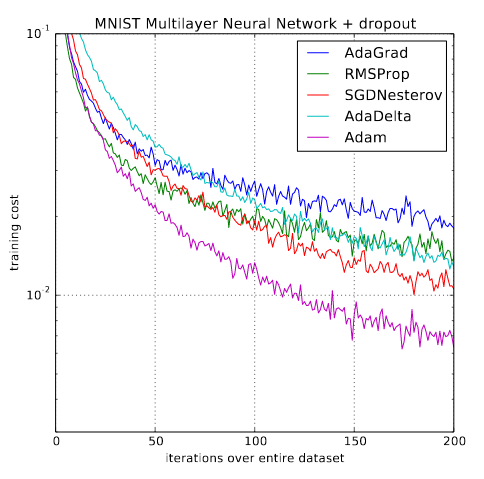
\includegraphics[width=0.3\linewidth]{figures/AdamGraph01}
		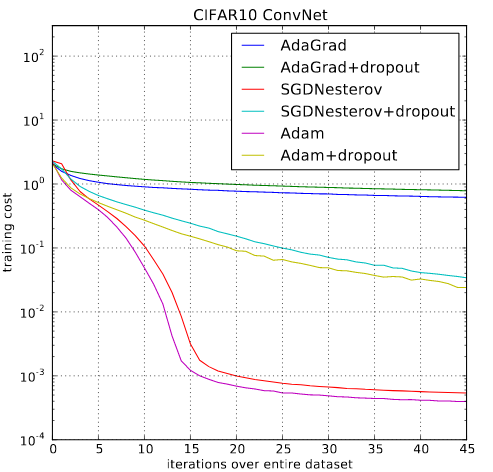
\includegraphics[width=0.3\linewidth]{figures/AdamGraph02}
		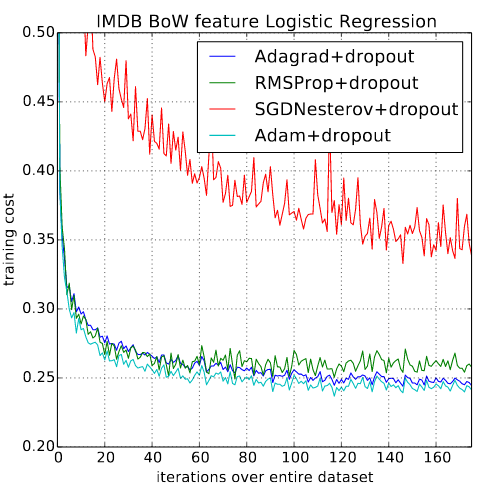
\includegraphics[width=0.3\linewidth]{figures/AdamGraph03}
		\caption[Adam teljesítménye a többi optimizáló algoritmushoz képest]{Adam teljesítménye a többi optimizáló algoritmushoz képest \cite{2014arXiv1412.6980K}}
		\label{fig:adamgraph}
	\end{figure}
	A hálózat optimalizálásához az Adam\cite{2014arXiv1412.6980K} algoritmust használtuk, mivel az általunk használt szakirodalom\cite{AdamTutorial1} ezt javasolta.
	Az Adam optimizer kombinálja az AdaGrad és RMSProp algoritmusokat, azaz paraméterenként különböző tanulási rátát használ, és ezeket a rátákat a nem régi gradiensek mérete alapján változtatja. Ezzel nagyobb hatékonyságot érve el, mint bármelyik alternatívája, ahogyan a mellékelt ábrán (\ref{fig:adamgraph}) is látható.
	\subsubsection{Lehetséges költségfüggvények}
	\paragraph{Sørensen–Dice tényező}
	\begin{equation}
	D = \frac {2*|{A \cap B}|}{|A|+|B|}
	\end{equation}
	A V-Net eredeti specifikációjában\cite{2016arXiv160604797M} ezt a loss algoritmust alkalmazták, és ez alapján jobb eredményeket értek el mint az alternatíváknál.
	\\[1em]
	Magát a tényezőt módosítás nélkül költségfüggvényként használni nem lehet, mivel a hálóban költségfüggvény minimalizálás történik, de ezt egyszerűen lehet orvosolni ha költségfüggvénynek a \(L = 1-D\)-t vesszük.
	\paragraph{Hausdorff távolság}
	\begin{equation}
	{d}_{H}(A,B)  = \max\left\{ \sup_{a\in A} \inf_{b\in B} {d}(a,b),\sup_{b\in B} \inf_{a\in A}{d}(a,b)\right\}
	\end{equation}
	A Hausdorff-távolság is használható költségfüggvényként, de mivel az eredeti specifikációban\cite{2016arXiv160604797M} csak kiértékelési szempontként szerepelt mi is így használtuk.
	\pagebreak
	\section{Eredmények}
	\subsection{Kiértékelési szempontok}
	Kiértékelési szempontként a már előbb említett költség függvényeken kívül figyelembe vettünk még további metrikákat is, amiknek alkalmazása nem lett volna megfelelő költségfüggvényként.
	\paragraph{Intersection over Union}
	\begin{equation}
	IoU = \frac{A\cap B} {A \cup B}
	\end{equation}
	Nagyon hasonló működésben a Dice tényezőhöz, de jóval szigorúbban értékeli a hamis pozitívokat. Sokkal kisebb probléma a jelen felhasználásnál, ha a máj mellett még minimális mennyiségű "test" is belekerül a szegmentációba, mintha máj maradna ki.
	\paragraph{Pixel Accuracy}
		\begin{equation}
	accuracy= \frac{TP+TN}{TP+TN+FP+FN}
	\end{equation}
	Ugyan fontos metrika kiértékelésnél, de költségfüggvényként való alkalmazása lehetetlen, mivel ha a két állapot kardinalitása közötti eltérés nagy, a hálózat lokális minimumba kerülhet, ezzel lassítva, vagy egyenesen lehetetlenné téve a konverganciát.
	\subsection{Kiértékelés}
\begin{figure}[!ht]
	\centering
	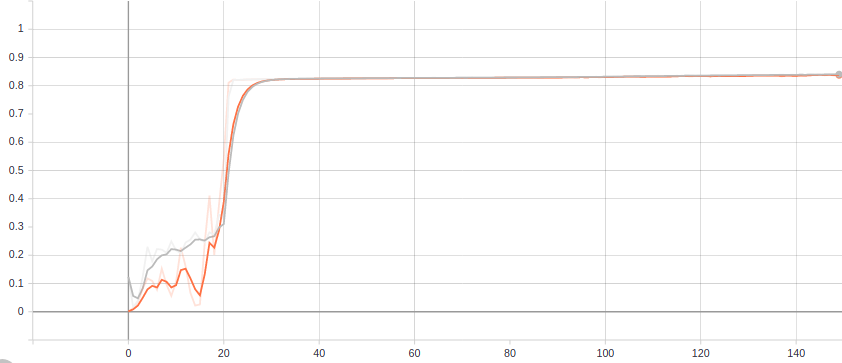
\includegraphics[width=0.35\linewidth]{figures/VNETAccuracy}
	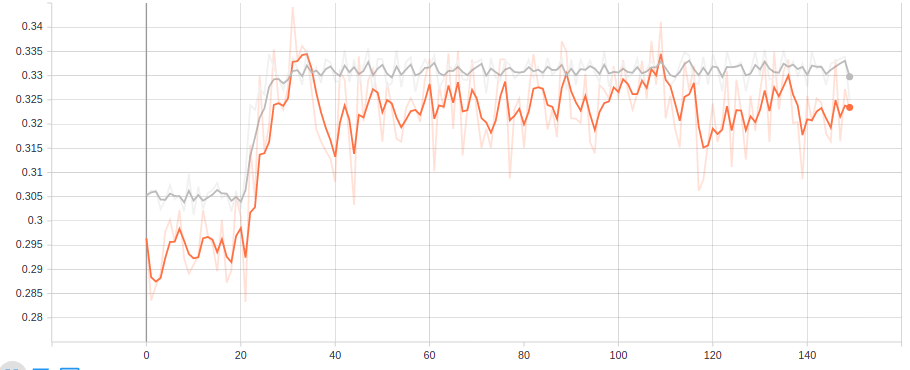
\includegraphics[width=0.35\linewidth]{figures/VNETDiceCoeff}
	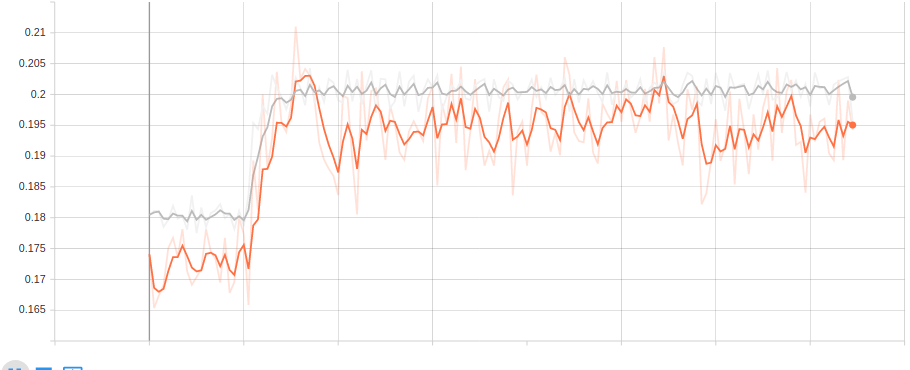
\includegraphics[width=0.35\linewidth]{figures/VNETIoUCoeff}
	\caption{A tanítás során keletkezett értékek, sorrendben Pixel pontosság, Dice együttható (költségfüggvény), IoU együttható}
	\label{fig:vnet}
\end{figure}
	A háló 150 epoch-on keresztül való tanítása után, 83\%-os pontosságot sikerült elérnünk.
Az ábrán (\ref{fig:vnet}) látható, hogy ugyan a háló konvergált, a "stabil" pont elérése után is rendkívül instabil a költségfüggvény. Ezt okozhatja a kiindulásnál megadott túl nagy tanulási ráta, vagy az általánosításhoz nem megfelelő mennyiségű adat.
\\[1em]
Összességében a képzett háló a körülményekhez képest jól működik, további adatokhoz való hozzáférés esetén értékei várhatóan javulnak. Az implementáció konfigurálhatósága miatt a paraméterekkel való további kísérletezésre is van lehetőség.
A kimeneti képek a \ref{fig:outputmask}. ábrán találhatóak.

	\begin{figure}[!h]
	\centering
	
\includegraphics[width=0.3\linewidth]{GoalMask}
	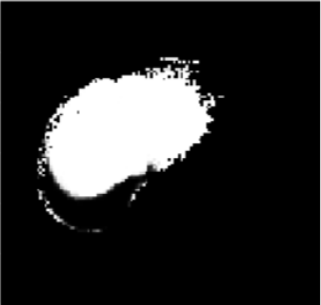
\includegraphics[width=0.32\linewidth]{PredictedMask}
	\caption{Az elkészül májszegmentáció, várt érték bal oldalt, kapott jobb oldalt}
	\label{fig:outputmask}
\end{figure}
	\section{További kutatási lehetőségek}
	Az adataugmentáció tovább fejleszthető a transzformációk biológiailag pontossá tevésével és a lineáris transzformációkon kívül esetleg elasztikus, vagy B-spline transzformációk alkalmazásával.
	A háló szempontjából hasznos lenne az eredmények más hálóknak ugyanarra az adathalmazra kapott eredményeivel való összehasonlítása, tanítás során drop layerek alkalmazása, kernelek paramétereinek változtatása, esetleg a háló mélységének növelése több GPU bevonásával.
	\section{Összefoglalás}
	A félév során megismerkedtünk a Python programozási nyelvvel és a Tensorflow keretrendszerrel, azon belül a tf.data és Keras API-kkal. Implementálásra került egy paraméterezhető V-Net architektúrát Keras segítségével megvalósító Python package és egy Nifti file-okat TFRecords-á átkonvertáló, majd ezek tf.data API-n keresztüli betöltését és transzformálását lehetővé tevő package. A félév során megismerkedtünk továbbá a neurális hálókkal, a deep learning fogalmával, a szegmentációs hálókkal, a V-Net-el és ennek lehetséges alternatíváival, a validáció, teszt és tanító adathalmazok elkülönítésének fontosságával, az iparban használt mérőszámokkal és ezek jelentésével, ezen kívül a TensorBoard alkalmazás használatával kiértékelés és ellenőrzés során. 
	\pagebreak
	\bibliography{bibliography}{}
	\bibliographystyle{ieeetr}
	
\end{document}